\documentclass[12pt, twoside]{article}
\usepackage[letterpaper, margin=1in, headsep=0.2in]{geometry}
\setlength{\headheight}{0.6in}
%\usepackage[english]{babel}
\usepackage[utf8]{inputenc}
\usepackage{microtype}
\usepackage{amsmath}
\usepackage{amssymb}
%\usepackage{amsfonts}
\usepackage{siunitx} %units in math. eg 20\milli\meter
\usepackage{yhmath} % for arcs, overparenth command
\usepackage{tikz} %graphics
\usetikzlibrary{quotes, angles}
\usepackage{graphicx} %consider setting \graphicspath{{images/}}
\usepackage{parskip} %no paragraph indent
\usepackage{enumitem}
\usepackage{multicol}
\usepackage{venndiagram}

\usepackage{fancyhdr}
\pagestyle{fancy}
\fancyhf{}
\renewcommand{\headrulewidth}{0pt} % disable the underline of the header
\raggedbottom
\hfuzz=2mm %suppresses overfull box warnings

\usepackage{hyperref}

\fancyhead[LE]{\thepage}
\fancyhead[RO]{\thepage \\ Name: \hspace{4cm} \,\\}
\fancyhead[LO]{BECA / Dr. Huson / Geometry\\*  Unit 8: Regents review\\* 7 March 2023}

\begin{document}

\subsubsection*{8.7 Classwork: Distance formula and Pythagorean theorem \hfill CCSSM}
\begin{enumerate}
\item In the diagram below of right triangle $ABC$, $AC=8$, and $AB=17$. Find the length $BC$ using the Pythagorean theorem.
\begin{flushright}
  \begin{tikzpicture}[scale=0.7]
  \draw [thick]
    (0,0)node[below]{$A$}--
    (-6,4)node[above]{$B$}--
    (-6,0)node[below]{$C$}--cycle;
    \draw (-6,0)++(0.5,0)--++(0,0.5)--+(-0.5,0);
    \node at (-3,0)[below]{$8$};
    \node at (-3,2.5){$17$};
\end{tikzpicture}
\end{flushright}

\item What is the distance between the points $(3,4)$ and $(6,8)$? \vspace{4cm}

\item Show that quadrilateral $ABCD$ is a rhombus by calculating the lengths of its sides. $A(0,3)$, $B(2,6)$, $C(4,3)$, $D(4,3)$
\begin{flushright}
  \begin{tikzpicture}[scale=0.6]
    \draw[help lines] (-2,-2) grid (6,8);
    \draw[thick, ->] (-2,0) -- (6.4,0) node [below right] {$x$};
    \draw[thick, <->] (0,-2.4)--(0,8.4) node [left] {$y$};
    \draw[thick] (0,3)node[left]{$A$}--
      (2,6)node[above]{$B$}--
      (4,3)node[right]{$C$}--
      (2,0)node[below]{$D$}--cycle;
  \end{tikzpicture}
\end{flushright}

\newpage
\item Rhombus $STAR$ has vertices $S(-1,2)$4, $T(2,3)$, $A(3,0)$, and $R(0,-1)$. What is the perimeter of rhombus $STAR$? \vspace{7cm}

\item The hypotenuse of right triangle $ABC$ is the radius of a circle centered at the origin, as shown. Use the lengths of the legs of the triangle and the Pythagorean formula to calculate the radius of the circle.
  \begin{flushright}
    \begin{tikzpicture}[scale=.635]
      %\draw [help lines] (-6,-6) grid (6,6);
      \draw [<->] (-6.5,0) -- (6.5,0) node [below right] {$x$};
      \draw [<->] (0,-6.5)--(0,6.5) node [left] {$y$};
      \draw (0,0) circle[radius=5];
        \fill (0,0) circle[radius=.1]node[below left]{$A$};
      \draw[thick] (0,0) -- (3,4)node[above right]{$B(3,4)$} -- (3,0)node[below right]{$C$} -- cycle;
      \draw (3,0)++(-.5,0)--++(0,.5)--++(.5,0);
    \end{tikzpicture}
  \end{flushright}


\end{enumerate}
\end{document}